\section{译者补充:经典电磁理论下的光学基础}\label{sec:译者补充:经典电磁理论下的光学基础}
\begin{remark}
    本节内容不是原书内容,而是译者根据《Optics》\citep{hecht2016optics}
    补充并参考\citet{OpticsChinese}翻译的,请酌情参考和斧正。
    本节内容只简要介绍相关基础概念和结论,
    并不像正式的物理和光学教材那样严谨,请读者批判性地看待本节内容。
    本节要求读者具备较好的微积分与电磁理论知识储备。
    此外读者需注意,本节遵循有关内容惯例采用右手坐标系,
    与正文pbrt采用的左手坐标系不同。
\end{remark}

\subsection{波动}\label{sub:波动}
光的本质是什么?光是波动现象还是粒子现象?
这个问题非常复杂。早在二十世纪,物理学家们就已经发现,
光的电磁理论的经典结论在微观层级上完全不成立。
然而当我们站在通常的大尺度视角下,电磁波及其经典理论已经够用了。
为了打好基础,我们从波的数学描述说起,它也适用于一切物理波。

\subsubsection*{一维波}
行进中的\keyindex{波}{wave}{}的一个本质特性是,
它是传播波的\keyindex{介质}{medium}{}的自持\keyindex{扰动}{disturbance}{}。
\keyindex{机械波}{mechanical wave}{wave\ 波}是
我们最熟悉的波,例如琴弦上的波、液体表面的波以及
空气中的\keyindex{声波}{sound wave}{wave\ 波}。
\begin{definition}[\keyindex{纵波}{longitudinal wave}{wave\ 波}]
    介质在波动方向上位移。
\end{definition}
\begin{definition}[\keyindex{横波}{transverse wave}{wave\ 波}]
    介质位移的方向垂直于波动方向。
\end{definition}
\begin{example}
    声波是纵波;琴弦上的波、电磁波是横波。
\end{example}
波区别于粒子流的几个关键特征之一是,
扰动在前进,但实物介质并不前进。
就像风吹起滚滚麦浪,但麦穗只是原地摇摆。
\begin{figure}[htbp]
    \centering
    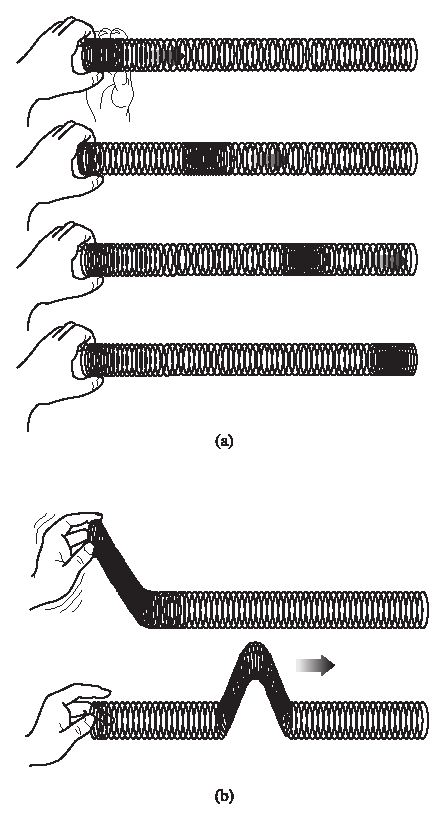
\includegraphics[width=0.65\linewidth]{Pictures/chap08/longitudinalAndTransverseWave.eps}
    \caption{弹簧中的(a)纵波;(b)横波。}
    \label{fig:08ex02.0201}
\end{figure}

我们暂不追究扰动的本质,而专注研究描述波动的方程应该具备怎样的形式。
设某个这样的扰动$\psi$以恒定速度$v$沿正$x$方向运动。
既然扰动在运动,则它必然是位置和时间的函数:
\begin{align}
    \psi(x,t)=f(x,t)\, ,
\end{align}
其中$f(x,t)$对应于某个具体函数或波形。
如\reffig{08ex02.0203}(a)所示,一个脉冲在静止坐标系$S$中以速度$v$运动。
我们取定任意时刻$t$即可得到那个时刻波的\keyindex{剖面}{profile}{},
就像脉冲经过时给它“拍照”。例如$t=0$有
\begin{align}
    \psi(x,t)\bigg|_{t=0}=f(x,0)=f(x)
\end{align}
表示0时刻波的剖面。
\begin{figure}[htbp]
    \centering
    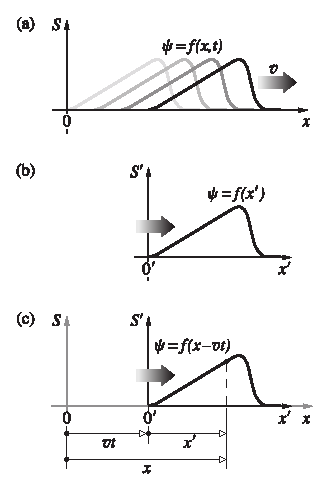
\includegraphics[width=0.5\linewidth]{Pictures/chap08/MovingReferenceFrame.eps}
    \caption{运动参考系。}
    \label{fig:08ex02.0203}
\end{figure}

现在,我们先只考虑传播时形状不变的波。
在一段时间$t$后,脉冲沿$x$轴前进了距离$vt$,其余不变。
如\reffig{08ex02.0203}(b),我们引入新坐标系$S'$并与脉冲以相同速度$v$运动。
则在该坐标系中$\psi$不再是时间的函数,而是静止不变的剖面,即
\begin{align}
    \psi=f(x')\, ,
\end{align}
这意味着坐标系$S'$中的扰动在任意时刻$t$的形状,
都和$S$中$t=0$时两者具有同一原点时扰动的形状相同,如\reffig{08ex02.0203}(c)所示。
为了将上式改写为$S$中某静止观察者描述的形式,我们利用
\begin{align}
    x'=x-vt
\end{align}
得到
\begin{align}
    \psi(x,t)=f(x-vt)\, .
\end{align}
上式是一维\keyindex{波函数}{wave function}{wave\ 波}的最一般形式。
它描述了一个具有所需剖面形状$f(x)$的波,它以速度$v>0$沿正$x$方向运动。
相似地,如果波向负$x$方向运动,则上式应改写为
\begin{align}
    \psi(x,t)=f(x+vt)\, .
\end{align}
总之变量$x$和$t$一定作为一个整体变量$x\mp vt$出现。

\subsubsection*{波动微分方程}
接下来我们推导一维波动方程的形式,把$\psi(x,t)$对空间与时间的依赖关系联系起来。注意到
\begin{align}
    \frac{\partial x'}{\partial x}=\frac{\partial (x\mp vt)}{\partial x}=1\, ,
\end{align}
以及
\begin{align}
    \frac{\partial x'}{\partial t}=\mp v\, ,
\end{align}
所以$\psi(x,t)$在$t$恒定时对$x$的偏微分为
\begin{align}
    \frac{\partial \psi}{\partial x}
    =\frac{\partial f}{\partial x}
    =\frac{\partial f}{\partial x'}\frac{\partial x'}{\partial x}
    =\frac{\partial f}{\partial x'}\, .
\end{align}
而在$x$恒定时$\psi(x,t)$对$t$的偏微分为
\begin{align}
    \frac{\partial \psi}{\partial t}
    =\frac{\partial f}{\partial t}
    =\frac{\partial f}{\partial x'}\frac{\partial x'}{\partial t}
    =\mp v\frac{\partial f}{\partial x'}
    =\mp v\frac{\partial \psi}{\partial x}\, .
\end{align}
上式表明$\psi$对$x$和$t$的变化率只差一个常系数。
继续求$\psi$的二阶偏微分有
\begin{align}
    \frac{\partial^2 \psi}{\partial x^2}
    =\frac{\partial}{\partial x}\left(\frac{\partial \psi}{\partial x}\right)
    =\frac{\partial}{\partial x}\left(\frac{\partial f}{\partial x'}\right)
    =\frac{\partial}{\partial x'}\left(\frac{\partial f}{\partial x'}\right)\frac{\partial x'}{\partial x}
    =\frac{\partial^2 f}{\partial x'^2}\, ,
\end{align}
并进一步得到
\begin{align}
    \frac{\partial^2 \psi}{\partial t^2}
    = & \frac{\partial}{\partial t}\left(\frac{\partial \psi}{\partial t}\right)
    =\frac{\partial}{\partial t}\left(\mp v\frac{\partial f}{\partial x'}\right)\nonumber    \\
    = & \mp v\frac{\partial}{\partial x'}\left(\frac{\partial f}{\partial t}\right)
    =\mp v\frac{\partial}{\partial x'}\left(\frac{\partial \psi}{\partial t}\right)\nonumber \\
    = & \mp v\frac{\partial}{\partial x'}\left(\mp v\frac{\partial f}{\partial x'}\right)
    =v^2\frac{\partial^2 f}{\partial x'^2}\nonumber                                          \\
    = & v^2\frac{\partial^2 \psi}{\partial x^2}\, .
\end{align}
整理上式即
\begin{definition}[一维\keyindex{波动微分方程}{differential wave equation}{equation\ 方程}]
    \begin{align}
        \frac{\partial^2 \psi}{\partial x^2}=\frac{1}{v^2}\frac{\partial^2 \psi}{\partial t^2}\, .
    \end{align}
\end{definition}
注意上式是一个\keyindex{齐次微分方程}{homogeneous differential equation}{equation\ 方程},
没有仅含独立变量的项(例如一份“力”或“源”),
所以描述的是\keyindex{无阻尼系统}{undamped system}{system\ 系统}。
这意味着若$\psi$是方程的解,则它乘以任意倍数后也是解。
反之,若一个波函数是上述方程的解,则它将是$x\mp vt$的函数,
且可以对$x$和$t$求得非平凡的二阶微分。

\subsubsection*{谐波}
最简单的波形是正弦或余弦曲线。它可以称作
\keyindex{正弦波}{sinusoidal wave}{wave\ 波}、
\keyindex{简谐波}{simple harmonic wave}{wave\ 波}
或\keyindex{谐波}{harmonic wave}{wave\ 波}。
任何波形都可以由谐波叠加合成。

我们为谐波波形选定为以下简单函数:
\begin{align}
    \psi(x,t)\bigg|_{t=0}=\psi(x)=f(x)=A\sin kx\, ,
\end{align}
其中常数$k>0$称作\keyindex{传播数}{propagation number}{},
$kx$这个整体是无量纲的。$\psi(x)$的最大值$A>0$称作波的\keyindex{振幅}{amplitude}{}。
将上式中的$x$替换为$x-vt$,改写成以速度$v$沿正$x$方向前进的波:
\begin{align}
    \psi(x,t)=A\sin k(x-vt) = f(x-vt)\, .
\end{align}
显然它是波动微分方程的一个解。该波在空间和时间中都具有周期性。
它的\keyindex{空间周期}{spatial period}{period\ 周期}
称作\keyindex{波长}{wavelength}{},表示每个波的长度,记作$\lambda$.
当$x$大小增减$\lambda$,$\psi$应不变:
\begin{align}
    \psi(x,t)=\psi(x\pm\lambda,t)\, .
\end{align}
这对应了正弦函数自变量改变$\pm2\pi$,由于$k>0,\ \lambda>0$,所以
\begin{align}
    \lambda=\frac{2\pi}{k}\, .
\end{align}

类似地,$\psi$的\keyindex{时间周期}{temporal period}{period\ 周期}记作$\tau$,
可简称\keyindex{周期}{period}{},即一个完整的波经过一静止观察者的时间。
它对应了波在时间上的重复行为:
\begin{align}
    \psi(x,t)=\psi(x,t\pm\tau)\, .
\end{align}
由此我们容易推出
\begin{align}
    kv\tau=2\pi\, ,
\end{align}
以及
\begin{align}
    \tau=\frac{\lambda}{v}\, .
\end{align}

周期的倒数称作\keyindex{时间频率}{temporal frequency}{frequency\ 频率},
可简称\keyindex{频率}{frequency}{},记作$\nu$,即单位时间里波的个数
\sidenote{注意$\nu$是希腊字母。}:
\begin{align}
    \nu=\frac{1}{\tau}\, ,
\end{align}
其单位为\keyindex{赫兹}{Hertz}{}(简写为Hz),即每秒周数。
结合前述定义,不难发现\keyindex{波速}{speed}{}$v$满足
\begin{align}
    v=\nu\lambda\, .
\end{align}

此外我们还定义\keyindex{时间角频率}{angular temporal frequency}{frequency\ 频率}为
\begin{align}
    \omega=\frac{2\pi}{\tau}=2\pi\nu=kv\, ,
\end{align}
可简称为角频率,单位为弧度每秒(rad/s)。

此外,\keyindex{空间频率}{spatial frequency}{frequency\ 频率},
也称\keyindex{波数}{wavenumber}{},定义为
\begin{align}
    \kappa=\frac{1}{\lambda}\, ,
\end{align}
即单位长度中波的数目,单位为$\mathrm{m}^{-1}$.

以上所有概念也适用于非谐波,只要它是由单个剖面元规则重复构成的。

利用以上定义,我们可以写出以下常见而等价的谐波表达式:
\begin{align}
    \psi= & A\sin k(x\mp vt)\, ,                                          \\
    \psi= & A\sin (kx\mp\omega t)\, ,                                     \\
    \psi= & A\sin 2\pi\left(\frac{x}{\lambda}\mp\frac{t}{\tau}\right)\, , \\
    \psi= & A\sin 2\pi(\kappa x\mp\nu t)\, ,                              \\
    \psi= & A\sin 2\pi\nu\left(\frac{x}{v}\mp t\right)\, ,
\end{align}
其中前两个最为常用,你甚至可以改用余弦函数来表示(后文就有)。
注意到这些理想化波的$x$和$t$没有取值范围限制,
又具有单一恒定频率,所以称作是\keyindex{单色的}{monochromatic}{}
或\keyindex{单能量的}{monoenergetic}{}。
但真实的波无法无限回溯到$t=-\infty$,所以不会是严格的单色波,而是含有一个频率范围。
若这个频段很窄,则称该波是\keyindex{准单色的}{quasimonochromatic}{}。

\subsubsection*{相位与相速度}
考察任一谐波,如
\begin{align}
    \psi(x,t)= & A\sin (kx-\omega t)\, ,
\end{align}
称正弦函数的整个输入值为波的\keyindex{相位}{phase}{},记作
\begin{align}
    \varphi=kx-\omega t\, .
\end{align}
更普遍地,对于谐波
\begin{align}
    \psi(x,t)= & A\sin (kx-\omega t+\varepsilon)\, ,
\end{align}
其相位为
\begin{align}
    \varphi=kx-\omega t+\varepsilon\, ,
\end{align}
其中$t=0$且$x=0$时的相位$\varepsilon$称作\keyindex{初相}{initial phase}{}。

根据相位定义,可知当$x$恒定时,相位对时间的变化率为
\begin{align}
    \left|\left(\frac{\partial\varphi}{\partial t}\right)_x\right|=\omega\, .
\end{align}
当$t$恒定时,相位对距离的变化率为
\begin{align}
    \left|\left(\frac{\partial\varphi}{\partial x}\right)_t\right|=k\, .
\end{align}
利用链式法则等微分知识,可推得
\begin{align}
    \left(\frac{\partial x}{\partial t}\right)_{\varphi}
    =-\displaystyle\frac{(\partial\varphi/\partial t)_x}
    {(\partial\varphi/\partial x)_t}
    =\pm\frac{\omega}{k}=\pm v\, .
\end{align}
上式最左边表示相位恒定状态的传播速度,称作波的\keyindex{相速度}{phase velocity}{}。
这里$v>0$,当波朝着正$x$方向运动时,则相速度取正号,反之则取负号。

\subsubsection*{叠加原理}
波动微分方程揭示了波一个明显区别于经典粒子流的性质:
\begin{theorem}[\keyindex{叠加原理}{Superposition Principle}{}]
    若$\psi_1$和$\psi_2$是同一波动方程的两个不同的解,
    则叠加它们的$\psi_1+\psi_2$也是一个解。
\end{theorem}
这意味着两个波到达同一片空间时会发生重叠,
简单地与另一方相加(相减),而不会永久瓦解其中某个波。
重叠区域内每一点的合扰动是该位置上单个成分波的代数之和。
在穿过共存区域后,每个波会继续前进离开,不受这次干扰。
注意这里我们讨论的是最为广泛的波的线性叠加,
暂不考虑极端情况下波的振幅大到以非线性方式驱动介质。

\begin{figure}[htb]
    \centering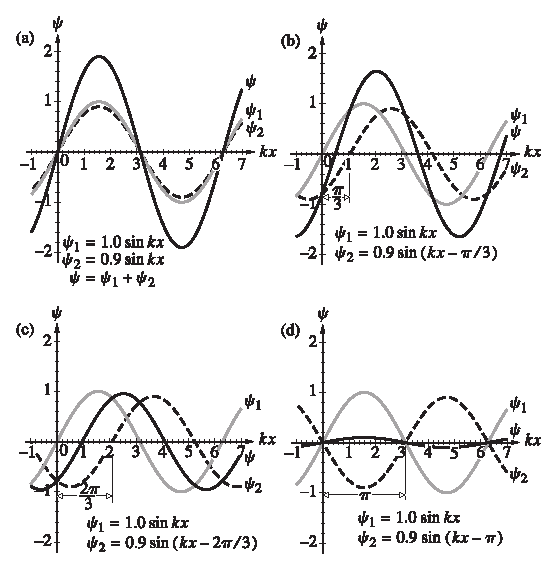
\includegraphics[width=0.9\linewidth]{Pictures/chap08/SuperpositionOfTwoSinusoids.eps}
    \caption{两个正弦波$\psi_1$和$\psi_2$的叠加,振幅分别为$A_1=1.0$和$A_2=0.9$.
        (a)$\psi_1$和$\psi_2$同相。(b)$\psi_1$领先$\psi_2$相角$\displaystyle\frac{\pi}{3}$.
        (c)$\psi_1$领先$\psi_2$相角$\displaystyle\frac{2\pi}{3}$.
        (d)$\psi_1$和$\psi_2$相位相差$\pi$,几乎要相互抵消。}
    \label{fig:08ex02.0216}
\end{figure}
\reffig{08ex02.0216}展示了两个振幅十分接近的波叠加后的结果与它们之间相位差的关系。
\reffig{08ex02.0216}(a)中两个波相位差为零,称为\keyindex{同相}{in-phase}{}。
它们互相加强,振幅增大,频率和波长不变。随着相位差增大,合成波振幅减小,
直到\reffig{08ex02.0216}(d)中相位差达到$\pi$,合成波几乎消失,
此时称两个波\keyindex{异相}{out-of-phase}{}
$180^\circ$.
异相波倾向于互相抵消的现象使得这整类现象被称作\keyindex{干涉}{interference}{}。

\subsubsection*{波的复数表示}
谐波所含的三角函数不便于数学处理,因此我们引入更方便的复数表示方法。
\keyindex{复数}{complex number}{}
$\widetilde{z}$形如
\begin{align}
    \widetilde{z}=x+\mathrm{i}y=r(\cos\theta+\mathrm{i}\sin\theta)=r\mathrm{e}^{\mathrm{i}\theta}\, ,
\end{align}
其中\keyindex{虚数单位}{imaginary unit}{}
$\mathrm{i}=\sqrt{-1}$.
实数$x$和$y$分别为$\widetilde{z}$的\keyindex{实部}{real part}{complex number\ 复数}
和\keyindex{虚部}{imaginary part}{complex number\ 复数};
实数$r\ge0$和$\theta$分别为$\widetilde{z}$的\keyindex{长度}{magnitude}{complex number\ 复数}
和\keyindex{相角}{phase angle}{complex number\ 复数};
长度也常记作$|\widetilde{z}|$,称为复数的\keyindex{模}{modulus}{complex number\ 复数}
或\keyindex{绝对值}{absolute value}{complex number\ 复数}。

本节中,复数的\keyindex{复共轭}{complex conjugate}{}用星号表示,即
\begin{align}
    \widetilde{z}^*=(x+\mathrm{i}y)^*=x-\mathrm{i}y
    =r(\cos\theta-\mathrm{i}\sin\theta)=r\mathrm{e}^{-\mathrm{i}\theta}\, .
\end{align}
于是复数的实部和虚部可以表示为
\begin{align}
    \mathrm{Re}(\widetilde{z})&=\frac{1}{2}(\widetilde{z}+\widetilde{z}^*)=r\cos\theta\, ,\\
    \mathrm{Im}(\widetilde{z})&=\frac{1}{2\mathrm{i}}(\widetilde{z}-\widetilde{z}^*)=r\sin\theta\, .
\end{align}
我们习惯上选用实部来描述谐波,即
\begin{align}
    \psi(x,t)=\mathrm{Re}[A\mathrm{e}^{\mathrm{i}(\omega t-kx+\varepsilon)}]\, ,
\end{align}
它等价于
\begin{align}
    \psi(x,t)=A\cos(\omega t-kx+\varepsilon)\, .
\end{align}
于是为了方便,在后文中我们略去实部记号把波函数简写为
\begin{align}
    \psi(x,t)=A\mathrm{e}^{\mathrm{i}(\omega t-kx+\varepsilon)}=A\mathrm{e}^{\mathrm{i}\varphi}\, ,
\end{align}
并借助复数运算法则(尤其是复指数乘除法的简便性)来进行计算,
只在要表示实际波时才取回实部。

要注意的是,波被表示为复数函数后,若参与了运算,
则只有当这些运算仅限于加减法、乘或除以一个实数,
或对一个实数变量进行微分或积分,才能恢复其实部,否则结果是错误的。

\subsubsection*{平面波}
给定时刻的光波可以用其频率、振幅、传播方向等描述,
但这并没有告诉我们光扰动在一片延伸的空间内的更多信息。
为此我们已经在定义\ref{definition:wavefront}中
引入了\keyindex{波阵面}{wavefront}{}
的概念。本节将研究理想的平面波的数学表达
\sidenote{本节向量等数学符号暂时遵循参考文献的记法。}。

\begin{figure}[htbp]
    \centering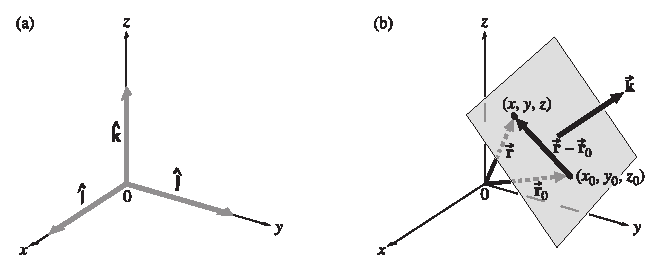
\includegraphics[width=\linewidth]{Pictures/chap08/CartesianUnitBasisVectors.eps}
    \caption{(a)直角坐标系单位基向量。(b)沿着$\vec{\mathbf{k}}$方向运动的平面波。}
    \label{fig:08ex02.0221}
\end{figure}
\keyindex{平面波}{plane wave}{wave\ 波}
是最简单的三维波了,其扰动的一切等相面构成一组平面,
且一般都垂直于传播方向。为此我们先给出平面的数学表达式:
如\reffig{08ex02.0221}(a)所示,对于直角坐标系中
的位置向量$\vec{\mathbf{r}}$,我们用三个坐标轴上的单位基向量来表示为
\begin{align}
    \vec{\mathbf{r}}=x\hat{\text{\sffamily\bfseries i}}+y\hat{\text{\sffamily\bfseries j}}+z\hat{\text{\sffamily\bfseries k}}\, .
\end{align}
它始于某个任意的原点$O$,止于点$(x,y,z)$,该点可以是空间中的任意位置。
类似地如\reffig{08ex02.0221}(b)所示,有
\begin{align}
    \vec{\mathbf{r}}-\vec{\mathbf{r}}_0
    =(x-x_0)\hat{\text{\sffamily\bfseries i}}+(y-y_0)\hat{\text{\sffamily\bfseries j}}+(z-z_0)\hat{\text{\sffamily\bfseries k}}\, .
\end{align}
我们令
\begin{align}
    (\vec{\mathbf{r}}-\vec{\mathbf{r}}_0)\cdot\vec{\mathbf{k}}=0\, ,
\end{align}
使得向量$\vec{\mathbf{r}}-\vec{\mathbf{r}}_0$扫过
一个垂直于$\vec{\mathbf{k}}$的平面,其端点$(x,y,z)$取一切允许的值。
设$\vec{\mathbf{k}}$为
\begin{align}
    \vec{\mathbf{k}}=k_x\hat{\text{\sffamily\bfseries i}}+k_y\hat{\text{\sffamily\bfseries j}}+k_z\hat{\text{\sffamily\bfseries k}}\, ,
\end{align}
则有
\begin{align}
    k_x(x-x_0)+k_y(y-y_0)+k_z(z-z_0)=0\, ,
\end{align}
即
\begin{align}
    k_xx+k_yy+k_zz=a\, ,
\end{align}
其中
\begin{align}
    a=k_xx_0+k_yy_0+k_zz_0=\text{常数}\, .
\end{align}
于是垂直于$\vec{\mathbf{k}}$的平面方程最简洁的表达形式为
\begin{align}
    \vec{\mathbf{k}}\cdot\vec{\mathbf{r}}=\text{常数}\, .
\end{align}
位置向量在$\vec{\mathbf{k}}$方向上的投影相同的所有点构成的轨迹即该平面。

\begin{figure}[htbp]
    \centering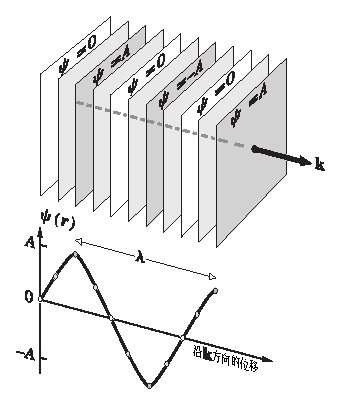
\includegraphics[width=0.5\linewidth]{Pictures/chap08/WavefrontsHarmonicPlaneWave.eps}
    \caption{平面简谐波的波阵面。}
    \label{fig:08ex02.0222}
\end{figure}
如\reffig{08ex02.0222},现在我们构建一组平面,
其上的$\psi(\vec{\mathbf{r}})$于空间中正弦地变化,即
\begin{align}
    \psi(\vec{\mathbf{r}})=&A\sin(\vec{\mathbf{k}}\cdot\vec{\mathbf{r}})\, ,\\
    \psi(\vec{\mathbf{r}})=&A\cos(\vec{\mathbf{k}}\cdot\vec{\mathbf{r}})\, ,\\
    \psi(\vec{\mathbf{r}})=&A\mathrm{e}^{\mathrm{i}\vec{\mathbf{k}}\cdot\vec{\mathbf{r}}}\, .
\end{align}
显然上面三个式子中,$\psi(\vec{\mathbf{r}})$都在
由$\vec{\mathbf{k}}\cdot\vec{\mathbf{r}}$取常数定义的每个平面上保持恒定。
沿着$\vec{\mathbf{k}}$方向位移$\lambda$后,$\psi$应当在空间中重复。
注意\reffig{08ex02.0222}中只画了无数平面中的若干个,
而平面本身也应无穷延伸,因为扰动充满整个空间。
当平面波在其波阵面上任意处均有相同“强度”时,
我们称其为\keyindex{均匀波}{homogeneous wave}{wave\ 波}。

总之,$\psi$在空间中的周期性可以表示为
\begin{align}
    \psi(\vec{\mathbf{r}})=\psi\left(\vec{\mathbf{r}}+\frac{\lambda\vec{\mathbf{k}}}{k}\right)\, ,
\end{align}
其中$k$是$\vec{\mathbf{k}}$的大小,
